\documentclass[]{article}


%\usepackage[sf,pagestyles,bf]{titlesec} % make section headings \sffamily
\usepackage{geometry}
\geometry{a4paper,portrait, 
 %margin=140pt,
 textwidth=455pt,
 lmargin=80pt,
 rmargin=80pt,
 tmargin=60pt,
 bmargin=60pt,
}
\usepackage{helvet}
\renewcommand{\familydefault}{\sfdefault}
\usepackage{amssymb,amsmath}
\usepackage{ifxetex,ifluatex}
\usepackage{fixltx2e} % provides \textsubscript
\ifnum 0\ifxetex 1\fi\ifluatex 1\fi=0 % if pdftex
  \usepackage[T1]{fontenc}
  \usepackage[utf8]{inputenc}
\else % if luatex or xelatex
  \usepackage{unicode-math}
  \defaultfontfeatures{Ligatures=TeX,Scale=MatchLowercase}
\fi
% use upquote if available, for straight quotes in Verbatim environments
\IfFileExists{upquote.sty}{\usepackage{upquote}}{}
% use microtype if available
\IfFileExists{microtype.sty}{%
\usepackage[]{microtype}
\UseMicrotypeSet[protrusion]{basicmath} % disable protrusion for tt fonts
}{}
\PassOptionsToPackage{hyphens}{url} % url is loaded by hyperref
\usepackage[unicode=true]{hyperref}
\hypersetup{
            pdftitle={Seminario de Investigación},
            pdfauthor={Lisandro Fernández},
            pdfborder={0 0 0},
            breaklinks=true}
\urlstyle{same}  % don't use monospace font for urls
\renewcommand\tabcolsep{4pt}
\usepackage{longtable,booktabs}
% Fix footnotes in tables (requires footnote package)
\IfFileExists{footnote.sty}{\usepackage{footnote}\makesavenoteenv{long table}}{}
\IfFileExists{parskip.sty}{%
\usepackage{parskip}
}{% else
\setlength{\parindent}{0pt}
\setlength{\parskip}{6pt plus 2pt minus 1pt}
}
\setlength{\emergencystretch}{3em}  % prevent overfull lines
\providecommand{\tightlist}{%
  \setlength{\itemsep}{0pt}\setlength{\parskip}{0pt}}
\setcounter{secnumdepth}{0}
% Redefines (sub)paragraphs to behave more like sections
\ifx\paragraph\undefined\else
\let\oldparagraph\paragraph
\renewcommand{\paragraph}[1]{\oldparagraph{#1}\mbox{}}
\fi
\ifx\subparagraph\undefined\else
\let\oldsubparagraph\subparagraph
\renewcommand{\subparagraph}[1]{\oldsubparagraph{#1}\mbox{}}
\fi

% set default figure placement to htbp
\makeatletter
\def\fps@figure{htbp}
\makeatother





\title{Seminario de Investigación}
\providecommand{\subtitle}[1]{}
\subtitle{Gramática Formal para Plan de Obra musical y Entorno de Secuenciación}
\author{Lisandro Fernández}
\date{Marzo 2019}

\usepackage{tikz} % insert this line
\usetikzlibrary{shapes,arrows,decorations.markings,positioning}

%\usepackage{listings}
%\usepackage{color}
%
%
%\lstset{
%  frame=tb,
%  language=Python,
%  aboveskip=3mm,
%  belowskip=3mm,
%  showstringspaces=false,
%  columns=flexible,
%  basicstyle={\small\ttfamily},
%  numbers=none,
%  numberstyle=\tiny\color{gray},
%  keywordstyle=\color{blue},
%  commentstyle=\color{dkgreen},
%  stringstyle=\color{mauve},
%  breaklines=true,
%  breakatwhitespace=true,
%  tabsize=3,
%  texcolor=red,
%}
\usepackage{color}
\usepackage[utf8]{inputenc}
\usepackage{fancyvrb}
 %\usepackage[usenames,dvipsnames]{xcolor}
\usepackage{xcolor}
\definecolor{dkgreen}{rgb}{0,0.6,0}
\definecolor{gray}{rgb}{0.5,0.5,0.5}
\definecolor{mauve}{rgb}{0.58,0,0.82}

\fvset{
	frame=single,
	framesep=1mm,
	fontfamily=courier,
	fontsize=\scriptsize,
	numbers=left,
	framerule=.3mm,
	numbersep=1mm,
	commandchars=\\\{\},
	rulecolor=\color{gray},
	label={Ejemplo:}
}

\begin{document}

% CARATULA

Alumno: Lisandro Fernández


Carrera:
Licenciatura en Música y Tecnología


Proyecto o programa acreditado en el que se inscribe el Seminario de Investigación: 
Cartografías Espacio-Temporales y Arte Sonoro



Profesor tutor: Pablo Riera

% TERMINA CARATULA

% \newpage

{
\setcounter{tocdepth}{3}

\renewcommand{\contentsname}{Contendios}
\tableofcontents
}
\hypertarget{resumen}{%
\subsection{1 Resumen}\label{resumen}}

El presente plan propone definir una gramática formal basada en texto
plano serializado\footnote{Coombs, Renear y De Rose (1987)} y
descriptivo, estructurada como árbol de análisis\footnote{Grela (1992)}
con el fin de representar planes de obra musical.

Acompañada por el desarrollo de un contexto de herramientas para
interprete de línea de comandos (Command Line Interface) para producción
de secuencias MIDI\footnote{Penfold (1992)} a partir de manipular
información subscripta a dicha representación.

El desarrollo se documentará\footnote{Kernighan y Plaguer (1978)
  Capítulo 8: Documentation (p.141-55)} para que su publicación cumpla
con las premisas del software libre.\footnote{Varios (2001)}

\newpage

\hypertarget{justificaciuxf3n}{%
\subsection{2 Justificación}\label{justificaciuxf3n}}

A continuación se argumentan los aspectos clave de este proyecto.

\hypertarget{por-quuxe9-texto-plano}{%
\subsubsection{2.1 ¿Por qué Texto Plano?}\label{por-quuxe9-texto-plano}}

\begin{quote}
``\ldots our base material isn't wood or iron, it's knowledge.
{[}\ldots{]}. And we believe that the best format for storing knowledge
persistently is plain text. With plain text, we give ourselves the
ability to manipulate knowledge, both manually and programmatically,
using virtually every tool at our disposal.'' (Hunt y Thomas 1999)
\end{quote}

\bigskip

Algunas ventajas del texto plano y legible en contraste a la
codificación de datos.\footnote{Hunt y Thomas (1999) Capítulo 3: Basic
  Tools (pp.~72-99).}

\textbf{Aprovechar.} Potencialmente cualquier herramienta de computo
puede operar información almacenada en texto plano.

\textbf{Mínimo Común Denominador.} Soportado en múltiples plataformas,
cada sistema operativo cuenta con al menos un editor de texto todos
compatibles hasta la codificación.

\textbf{Fácil de manipular.} Procesar cadenas de caracteres es de los
trabajos mas rudimentales que pueden ser realizados por un sistema
informático.

\textbf{Fácil de mantener.} El texto plano no presenta ninguna
dificultad o impedimento ante la necesidad de actualizar información o
de realizar cualquier tipo de cambio o ajuste.

\textbf{Fácil de comprobar.} Es sencillo agregar, actualizar o modificar
datos de testeo sin la necesidad de emplear o desarrollar herramientas
especiales para ello.

\textbf{Liviano.} Determinante cuando los recursos de sistema son
limitados como por ejemplo almacenamiento escaso, velocidad de computo
restringida o conexiones lentas.

\textbf{Seguro contra toda obsolescencia (o compatible con el avance).}
Los archivos de datos en formatos legibles y autodescriptivos perduran
por sobre otros formatos aun cuando caduquen las aplicaciones con las
hayan sido creados.\footnote{Leek (2017)}

\hypertarget{por-quuxe9-interfaz-de-linea-de-comandos}{%
\subsubsection{2.2 ¿Por qué Interfaz de Linea de
Comandos?}\label{por-quuxe9-interfaz-de-linea-de-comandos}}

\textbf{Primer estado operativo de un ordenador.} Eventualmente todos
los sistemas operativos permiten ser utilizados a través de este acceso
previo al gerente de escritorio.

\textbf{Menor utilización de recursos.} No depender de un agente de
ventanas interviniendo entre el usuario y el sistema libra una cantidad
considerable de recursos.

\textbf{Una interfaz para diferentes aplicaciones.} La estructura de las
instrucciones para esta interfaz \emph{aplicación - argumento - recurso}
(su analogía \emph{verbo - adverbio - sujeto}) persiste para cualquier
pieza de software. Dicha recurrencía elimina el ejercicio que significa
operar de modo distinto cada aplicación, permitiendo un accionar
semejante en contextos y circunstancias diferentes.

\textbf{Tradición.} Perdura por décadas como estándar durante la
historia de la informática remitiendo a los orígenes de los ordenadores
basados en teletipo.

\textbf{Resultados reproducibles.} Si bien la operación de sistemas sin
mas que la entrada de caracteres requiere conocimiento y entrenamiento
específico, no considerar la capa que representa la posición del puntero
como parámetros de instrucciones, permite que sean recopiladas en
secuencias de acciones precisas (guión).

\textbf{Pipeline y Automatización.} La composición flujos de procesos
complejos encadenando resultados con trabajos.\footnote{Raymond (1999)
  Capítulo 1: Context, Apartado 1: Philosophy, Sub-apartado: Basics of
  the Unix Philosophy (pp.~34-50)}

\textbf{Acceso remoto.} Mas allá del protocolo en el que se base la
negociación local/remoto la interfaz de linea comandos es la herramienta
de facto para administrar un sistema a distancia.

\textbf{Productividad.} Valerse de herramientas pulidas como editores de
texto avanzados (VIM / Emacs) que gracias al uso de atajos (acciones
complejas asignadas a combinaciones de teclas) evitan la alternancia
entre mouse y teclado, lo cual promueve un flujo de trabajo
ágil.\footnote{Moolenaar (2000)}

\hypertarget{objetivos}{%
\subsection{3 Objetivos}\label{objetivos}}

Este proyecto procura establecer un contexto y proveer los recursos para
un procedimiento sencillo y flexible de elaboración discursos musicales
unificando la planificación de obra con la secuenciación MIDI.

Ademas pretende exponer las ventajas de la Interfaz de Linea de Comandos
para operar sistemas informáticos a la comunidad de artistas, teóricos e
investigadores.

Promover la adopción de prácticas consolidadas y formatos abiertos para
representar, manipular y almacenar información digital.

Fomentar el trabajo colaborativo generando vínculos con y entre
usuarios.\footnote{Raymond (1997) Capítulo 11: The Social Context of
  Open-Source Software (p.~11)}\footnote{Yzaguirre (2016)}

\newpage

\hypertarget{marco-referencial}{%
\subsection{4 Marco referencial}\label{marco-referencial}}

A continuación se describen algunos desarrollos que vinculan
representación y manipulación de información musical: MuseData, Humdrum,
MusicXML y MML; como ejemplo de un marco de programación basada en una
sintaxis declarativa se cosideró Flocking.

\hypertarget{musedata}{%
\subsubsection{4.1 MuseData}\label{musedata}}

La base de datos MuseData\footnote{Selfridge-Field (1997)} es un
proyecto y a la vez el sistema de codificación principal del Centro de
Investigación Asistida por Computador en Humanidades (CCARH). La base de
datos fue creado por Walter Hewlett.

Los archivos MuseData tienen el potencial de existir en múltiples
formatos comunes de información. La mayoría de las codificaciones
derivadas acomodan sólo algunas de las las características incluidas en
el master MuseData de codificaciones. El archivo MuseData está diseñado
para soportar aplicaciones de sonido, gráficos y análisis. Los formatos
derivados de las codificaciones musicales de MuseData que se
distribución son: MIDI1, MIDI+ y Humdrum.

\hypertarget{organizaciuxf3n-de-archivos-musedata}{%
\paragraph{4.1.1 Organización de archivos
MuseData}\label{organizaciuxf3n-de-archivos-musedata}}

Los archivos MuseData están basados en ASCII y se pueden ver en
cualquier editor de texto. Dentro del formato MuseData El número de
archivos por movimiento y por trabajo puede variar de un formato a otro
así como también de una edición a otra.

Los archivos MuseData están organizados en base a las partes. Un
movimiento de una composición es típicamente encontrado dividido en
varios archivos agrupados en un directorio para ese movimiento.

Las partes de los archivos MuseData siempre tienen la etiqueta 01 para
la primera parte, 02 para la segunda parte de la partitura, etc.
Conteniendo varias líneas de música, como dos flautas en una partitura
de orquesta, o dos sistemas para música de piano. Archivos para
diferentes los movimientos de una composición se encuentran en
directorios separados que usualmente indican el número de movimiento,
p.~01, 02, etc.

La exhaustividad de la información dentro de los archivos varía entre
dos niveles que en archivos MuseData llamamos Stage 1 y Stage 2. Sólo
los archivos Stage 2 son recomendados para aplicaciones serias.

El primer paso en la entrada de datos (Stage 1) captura información
básica como duración y altura de las notas. Por ejemplo, normalmente
habría cuatro archivos (Violín 1, Violín 2, Viola, Violonchelo) para
cada movimiento de un cuarteto de cuerdas. Si el movimiento del cuarteto
comienza en metro binario, cambia a metro ternario, y luego vuelve a
binario, cada sección métrica tendrá su propio conjunto de partes. Así
habría doce archivos para el movimiento. El segundo paso en la entrada
de datos (Stage 2) suministra toda la información que no puede ser
capturado de forma fiable desde un teclado electrónico. Esto incluye
indicaciones para ritmo, dinámica y articulación.

El juicio humano se aplica en el Stage 2. Así, cuando el movimiento del
cuarteto de cuerdas citado anteriormente se convierte a la Stage 2, las
tres secciones métricas para cada instrumento capturado desde la entrada
del teclado se encadenará en un movimiento cada uno. El movimiento
tendrá ahora cuatro archivos de datos (uno para Violín 1, otro para
Violín 2, Viola, Violonchelo).

El juicio humano también proporciona correcciones y anotaciones a los
datos. Algunos tipos de errores (por ejemplo, medidas incompletas) deben
corregirse y así consiguen tener sentido para el usuario. Los asuntos
que son más discrecionales (tales como alteraciones opcionales de los
ornamentos o accidentes) por lo general no se modifica. Las decisiones
discrecionales se anotan en archivos que permiten marcas editoriales.

\hypertarget{la-representaciuxf3n-musedata-de-informaciuxf3n-musical}{%
\paragraph{4.1.2 La representación MuseData de información
musical}\label{la-representaciuxf3n-musedata-de-informaciuxf3n-musical}}

El propósito de la sintaxis MuseData es representar el contenido lógico
de una pieza musical de una modo neutral. El código se utiliza
actualmente en la construcción de bases de datos de texto completo de
música de varios compositores, J.S. Bach, Beethoven, Corelli, Handel,
Haydn, Mozart, Telemann y Vivaldi. Se pretende que estas bases de datos
de texto completo se utilicen para la impresión de música, análisis
musical y producción de archivos de sonido digitales.

Aunque el código MuseData está destinado a ser genérico, se han
desarrollado piezas de software de diversos tipos con el fin de probar
su eficacia. Las aplicaciones MuseData pueden imprimir resultados y
partes para ser utilizadas por editores profesionales de música, así
como también compilar archivos MIDI (que se pueden utilizar con
secuenciadores estándar) y facilitar las búsquedas rápidas de los datos
de patrones rítmicos, melódicos y armónicos específicos.

La sintaxis MuseData está diseñada para representar tanto información de
notación como de sonido, pero en ambos casos no se pretende que la
representación esté completa. Eso prevé que los registros MuseData
servirían como archivos de origen para generar tanto documentos gráficos
(específicamente de página) y archivos de performance MIDI, que podrían
editarse como el usuario lo crea conveniente. Las razones de esta
postura son dos:

\begin{itemize}
\item
  Cuando se codifica una obra musical, no es la partitura sino el
  contenido lógico de la partitura lo que codifica. Codificar la
  puntuación significaría codificar la posición exacta de cada nota en
  la página; pero nuestra opinión es que tal codificación realmente
  contendría más información que la que el compositor pretende
  transmitir.
\item
  No se puede anticipar todos los usos a los cuales podrían darse estos
  datos, pero se pude estar bastante seguro de que cada usuario tendrá
  sus propias necesidades especiales y preferencias. Por lo tanto, no
  tiene sentido tratar de codificar información acerca de cómo debe
  verse una realización gráfica de los datos o cómo sonido que estos
  datos representan debe sonar.
\end{itemize}

Por otro lado, a veces puede ser útil hacer sugerencias sobre cómo los
gráficos y el sonido deben ser realizados. Lo importante es identificar
las sugerencias como un tipo de datos independiente, que puede ser
fácilmente ignorado por software de aplicación o despojado enteramente
de los datos. MuseData software usa estas sugerencias de impresión y
sonido en el proceso de generación de documentos de partitura y archivos
MIDI.

\hypertarget{humdrum}{%
\subsubsection{4.2 Humdrum}\label{humdrum}}

David Huron creó Humdrum\footnote{Wild (1996)} en los años 80, y se ha
utilizado constantemente por décadas. Humdrum es un conjunto de
herramientas de línea de comandos que facilita el análisis, así como una
sintaxis generalizada para representar secuencias de datos. Debido a que
es un conjunto de herramientas de línea de comandos, es el lenguaje de
programa agnóstico. Muchos han empleado herramientas de Humdrum en
secuencias de comandos más grandes que utilizan PERL, Ruby, Python,
Bash, LISP y C++.

\hypertarget{representaciuxf3n}{%
\paragraph{4.2.1 Representación}\label{representaciuxf3n}}

En primer lugar, Humdrum define una sintaxis para representar
información discreta como una serie de registros en un archivo de
computadora.

\begin{itemize}
\item
  Su definición permite que se codifiquen muchos tipos de información.
\item
  El esquema esencial utilizado en la base de datos CCARH para la altura
  y la duración musical es sólo uno de un conjunto abierto.
\item
  Algunos otros esquemas pueden ser aumentados por gramáticas definidas
  por el usuario para tareas de investigación.
\end{itemize}

\hypertarget{manipulaciuxf3n}{%
\paragraph{4.2.2 Manipulación}\label{manipulaciuxf3n}}

Segundo, está el conjunto de comandos, el Humdrum Toolkit, diseñado para
manipular archivos que se ajusten a la sintaxis Humdrum en el campo de
la investigación asistida por ordenador en la música.

El énfasis está en \textbf{asistido}:

\begin{itemize}
\item
  Humdrum no posee facultades analíticas de nivel superior per se.
\item
  Más bien, \emph{su poder deriva de la flexibilidad de su kit de
  elementos, utilizados en combinacióin} para explotar plenamente el
  potencial del sistema.
\end{itemize}

\hypertarget{de-la-experiencia-a-la-apreciaciuxf3n}{%
\paragraph{4.2.3 De la experiencia a la
apreciación}\label{de-la-experiencia-a-la-apreciaciuxf3n}}

Apreciación de todo el potencial de Humdrum es definitivamente a partir
de la experiencia. En palabras de David Huron:

\begin{quote}
Cualquier conjunto de herramientas requiere el desarrollo de una
experiencia concomitante, y Humdrum Toolkit no es una excepción. Espero
que la inversión de el tiempo requerido para aprender a usar Humdrum
será más que compensado por ganancias académicas posteriores.
\end{quote}

Los usuarios de Humdrum hasta ahora han tendido a trabajar en la
percepción de la música o etnomusicología, mientras que los teóricos y
los musicólogos histioriadores han sido lentos para reconocer el
potencial del sistema.

\hypertarget{cli-vs-gui}{%
\paragraph{4.2.4 CLI vs GUI}\label{cli-vs-gui}}

Humdrum u otros sistemas como él ofrecen los recursos para una marcar un
paradigma para la investigación musical.

El tedio de recopilar pruebas sólidas que apoyen las propias teorías
pueden ser aliviadas por la automatización, y cuanto mayor sea la
cantidad de música examinada mayor será el rigor de la prueba de las
hipótesis.

Sin embargo, la desafortunada posibilidad es que muchos de los
musicólogos y teóricos que se benefician de una pequeña intuición
asistida por la máquina es probable que sean repelidos por la interfaz
totalmente basada en texto de Humdrum.

Aunque en el análisis final los comandos estilo UNIX son seguramente más
flexibles y eficientes que una interfaz gráfica ``amigable'', pueden
parecer intimidantes para no programadores, muchos de los cuales pueden
ser disuadidos de hacer uso de un herramienta de otra manera valiosa.

Independientemente de que los teóricos de la música decidan o no
aumentar su invaluable intuición musical con valiosas pruebas empíricas,
los resultados basados en las cantidades máximas de datos pertinentes
será un factor en la evolución de nuestra disciplina.

\hypertarget{musicxml}{%
\subsubsection{4.3 MusicXML}\label{musicxml}}

MusicXML\footnote{Good (2001)} fue diseñado desde cero para compartir
archivos de música entre aplicaciones y para archivar registros de
música para uso en el futuro. Se puede contar con archivos de MusicXML
que son legibles y utilizables por una amplia gama de notaciones
musicales, ahora y en el futuro. MusicXML complementa al los formatos de
archivo utilizados por Finale y otros programas.

MusicXML se pretende un el estándar para compartir partituras
interactivas, dado que facilita crear música en un programa y exportar
sus resultados a otros programas. Al momento más de 220 aplicaciones
incluyen compatibilidad con MusicXML.

\hypertarget{music-markup-language}{%
\subsubsection{4.4 Music Markup Language}\label{music-markup-language}}

El Lenguaje de Marcado de Música (MML)\footnote{Steyn (2001)} es un
intento de marcar objetos y eventos de música con un lenguaje basado en
XML. La marcación de estos objetos debería permitir gestionar la música
documentos para diversos fines, desde la teoría musical y la notación
hasta rendimiento práctico. Este proyecto no está completo y está en
progreso. El primer borrador de una posible DTD está disponible y se
ofrecen algunos ejemplos de piezas de música marcadas con MML.

El enfoque es modular. Muchos módulos aún están incompletos y necesitan
más investigación y atención.

Si una pieza musical está serializada usando MML puede ser entregada en
al menos los siguientes formatos:

\begin{itemize}
\item
  Texto: representación de notas como, por ejemplo, piano-roll (como el
  que se encuentra en el software del secuenciador de computadora)
\item
  Common Western Notation: Notación musical occidental en pantalla o en
  papel
\item
  MIDI-device: MML hace posible ``secuenciar'' una pieza de música sin
  tener que usar software especial. Así que cualquier persona con un
  editor de texto debe ser capaz de secuenciar la música de esta manera.
\end{itemize}

\hypertarget{flocking}{%
\subsubsection{4.5 Flocking}\label{flocking}}

Flocking\footnote{Clark y Tindale (2014)} es un framework, escrito en
JavaScript, para la composición de música por computadora que aprovecha
las tecnologías e ideas existentes para crear un sistema robusto,
flexible y expresivo. Flocking combina el patrón generador de unidades
de muchos idiomas de música de computadora con tecnologías Web Audio
para permitir a los usuarios interactuar con sitios Web existentes y
potenciales tecnologías. Los usuarios interactúan con Flocking usando un
estilo declarativo de programación.

El objetivo de Flocking es permitir el crecimiento de un ecosistema de
herramientas que puedan analizar y entender fácilmente la lógica y la
semántica de los instrumentos digitales representando de forma
declarativa los pilares básicos de síntesis de audio. Esto es
particularmente útil para soportar la composición generativa (donde los
programas generan nuevos instrumentos y puntajes de forma algorítmica),
herramientas gráficas (para que programadores y no programadores
colaboren), y nuevos modos de programación social que permiten a los
músicos adaptar, ampliar y volver a trabajar fácilmente en instrumentos
existentes.

\hypertarget{como-funciona-flocking}{%
\paragraph{4.5.1 Como funciona Flocking}\label{como-funciona-flocking}}

El núcleo del framework Flocking consiste en varios componentes
interconectados que proporcionan la capacidad esencial de interpretar e
instanciar generadores de unidades, producir flujos de muestras y
programar procesos. Los principales componentes de Flocking incluyen:

\begin{enumerate}
\def\labelenumi{\arabic{enumi}.}
\item
  el \emph{Intérprete Flocking}, que analiza e instancia sintetizadores,
  generadores de unidad y bufers
\item
  el \emph{Ecosistema}, que representa el audio general y su
  configuración
\item
  \emph{Audio Strategies}, que son las salidas de audio conectables
  (vinculados a los backends como la API de audio web o ALSA en Node.js)
\item
  \emph{Unit Generators} (ugens), que son funciones primitivas
  generadoras de las muestras utilizadas para producir sonido
\item
  \emph{Synths} (sintetizadores) que representan instrumentos y
  colecciones en la lógica de generación de señales
\item
  el \emph{Scheduler} (programador ó secuenciador), que gestiona el
  cambio secunecial (basado en el tiempo) eventos en un sintetizador
\end{enumerate}

\hypertarget{programaciuxf3n-declarativa}{%
\paragraph{4.5.2 Programación
declarativa}\label{programaciuxf3n-declarativa}}

Arriba, se describió Flocking como un marco \textbf{declarativo}. Esta
característica es esencial para comprender su diseño. La programación
declarativa se puede entender en el contexto de Flocking por dos
aspectos esenciales:

\begin{enumerate}
\def\labelenumi{\arabic{enumi}.}
\item
  enfatiza una visión semántica de alto nivel de la lógica y estructura
  de un programa
\item
  representa los programas como estructuras de datos que pueden ser
  entendido por otros programas.
\end{enumerate}

El énfasis aquí es sobre los aspectos lógicos o semánticos de la
computación, en vez de en la secuenciación de bajo nivel y el flujo de
control. Tradicionalmente los estilos de programación imperativos suelen
estar destinados solo para el compilador. Aunque el código es a menudo
compartido entre varios desarrolladores, no suele ser comprendidos o
manipulados por programas distintos a los compiladores.

Por el contrario, la programación declarativa implica la capacidad de
escribir programas que están representados en un formato que pueden ser
procesados por otros programas como datos ordinarios. La familia de
lenguajes Lisp es un ejemplo bien conocido de este enfoque. Paul Graham
describe la naturaleza declarativa de Lisp, expresando que ``no tiene
sintaxis. Escribes programas en árboles de análisis\ldots{} {[}que{]}
son totalmente accesibles a tus programas. Puedes escribir programas que
los manipulen\ldots{} programas que escriben programas''.\footnote{Graham
  (2001)} Aunque Flocking está escrito en JavaScript, comparte con Lisp
el enfoque expresar programas dentro de estructuras de datos que estén
disponibles para su manipulación por otros programas.

\newpage

\hypertarget{metodologuxeda}{%
\subsection{5 Metodología}\label{metodologuxeda}}

\hypertarget{hipuxf3tesis-de-trabajo}{%
\subsubsection{5.1 Hipótesis de trabajo}\label{hipuxf3tesis-de-trabajo}}

El entorno de producción musical que se pretende establecer estará
principalmente integrando por:

El estandar YAML\footnote{Varios (2018c)} como opción para serializar
las definiciones de cada parte instrumental.

La rutina de instrucciones principales será interpretada en el lenguaje
Python\footnote{Rossum (2018)} (en su ultima versión estable). Esta
pieza de software estará basada en otros dos desarrollos: el módulo
``\emph{pyyaml}''\footnote{Varios (2018a)} para analizar la información
serializada, en combinación con la librería ``\emph{music21}''\footnote{Cuthbert
  (2018)} que asistirá en las tareas de musicología. Ademas se
incorporan algunos módulos de la ``\emph{Librería Estandar}'',\footnote{Varios
  (2018b)} mientras que la documentación se generará con
``\emph{sphinx}''.\footnote{Brandl y Sphinx team (2018)}

El editor de texto preferido para toda la actividad será VIM;\footnote{Moolenaar
  (2018)} durante el desarrollo las versiones se controlarán con el
sistema GIT\footnote{Torvalds (2018)} y el repositorio del proyecto se
almacenará en un espacio online proveido por algún servicio del tipo
GitLab.

\hypertarget{actividades-de-investigaciuxf3n}{%
\subsubsection{5.2 Actividades de
investigación}\label{actividades-de-investigaciuxf3n}}

\begin{center}
    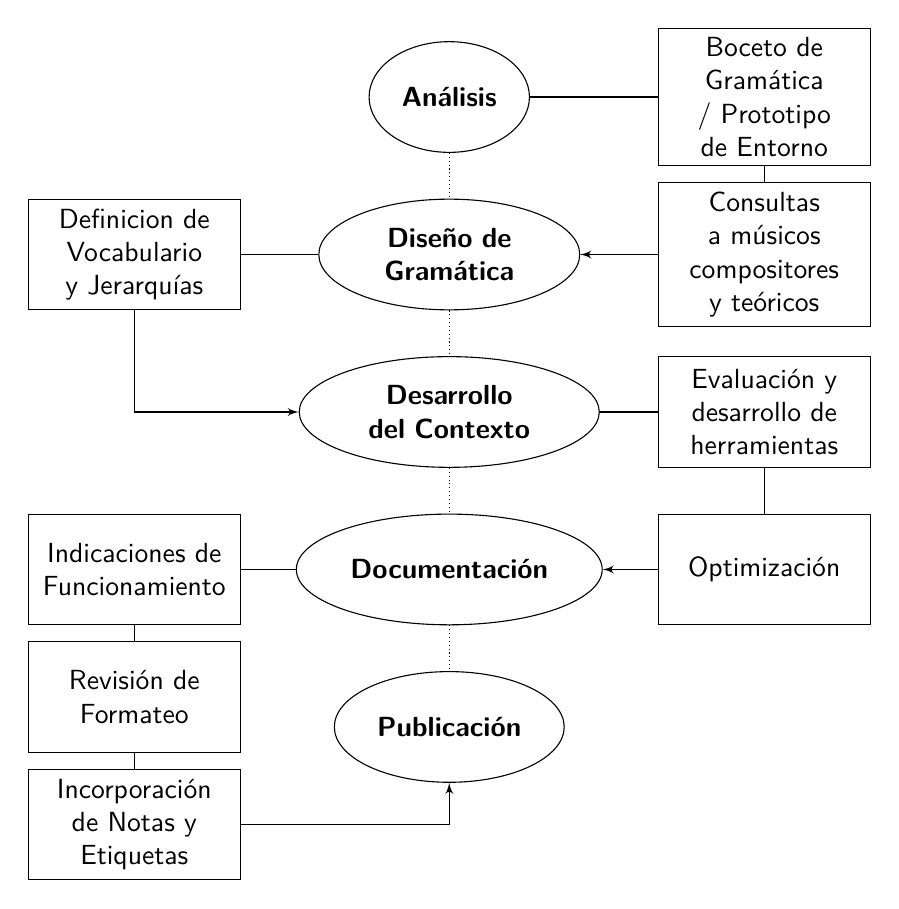
\begin{tikzpicture}[node distance = 2cm, auto]

    \tikzstyle{circulo} = [
        ellipse, 
        draw, 
        %fill=red!20, 
        minimum height=4em,
        text centered, 
        node distance=2cm,
    font=\bfseries
    ]
    \tikzstyle{block} = [
        rectangle, 
        draw, 
        %fill=blue!20, 
        text width=7em, 
        text centered, 
        minimum height=4em,
        node distance=2cm,
    ]
    \tikzstyle{line} = [
        draw,
        -latex',
    ]

    %\tikzset{flecha/.style={
    %    decoration={
    %       markings,mark=at position 1 with %
    %       {\arrow[scale=3,>=stealth]{>}}},
    %       postaction={decorate}
    %    }
    %}
    \node [circulo]              (ana) {Análisis};
    \node [circulo, text width=6em,below of=ana](dis) {Diseño de Gramática};
    \node [circulo, text width=7em, below of=dis](dev) {Desarrollo del Contexto};
    \node [circulo, below of=dev](doc) {Documentación};
    \node [circulo, below of=doc](dep) {Publicación};

    %\path [line] (ana) -- (dis) -- (dev) -- (doc) -- (dep);
    \draw[densely dotted] (ana) -- (dis);
    \draw[densely dotted] (dis) -- (dev);
    \draw[densely dotted] (dev) -- (doc);
    \draw[densely dotted] (doc) -- (dep);

    \node [block, 
        right of=ana,
        node distance=4cm,
    ](boc) { 
          Boceto de Gramática
          / Prototipo de Entorno
    };


    \node [block, 
        below of=boc
    ](enc) { 
          Consultas a músicos compositores y teóricos
    };

    \path [line] (ana) -- (boc) -- (enc) -- (dis);







    \node [block, 
        left of=dis,
        node distance=4cm,
    ](def) { 
    Definicion de Vocabulario y Jerarquías
    };

    %\node [block, 
    %    below of=def
    %](sin) { 
    %      Sintaxis YAML
    %};

    \path [line] (dis) -- (def) |-  (dev) ;


      

    \node [block, 
        right of=dev,
        node distance=4cm,
    ](per) { 
      Evaluación y desarrollo de herramientas
    };


    \node [block, 
        below of=per
    ](opt) { 
      Optimización
    };

    \path [line] (dev) -- (per) -- (opt) -- (doc);



    \node [block, 
        left of=doc,
        node distance=4cm,
    ](fun) { 
    Indicaciones de Funcionamiento
    };

    \node [block, 
    below = 0.2cm of fun
    ](for) { 
    Revisión de Formateo 
    };
    \node [block, 
    below = 0.2cm of for
    ](not) { 
    Incorporación de Notas y Etiquetas 
    };

    \path [line] (doc) -- (fun) -- (for) -- (not) -| (dep) ;

     \end{tikzpicture}
     
\end{center}

\newpage

\hypertarget{cronograma-de-trabajo}{%
\subsection{6 Cronograma de Trabajo}\label{cronograma-de-trabajo}}

\begin{longtable}[]{@{}lll@{}}
\toprule
& Tiempo estipulado & Fechas tentativas\tabularnewline
\midrule
\endhead
Boceto de gramática & 6 semanas & Septiembre y octubre del
2018\tabularnewline
Prototipo de entorno & 6 semanas & Octubre y noviembre del
2018\tabularnewline
Entrevistas y consultas & 4 semanas & Diciembre del 2018\tabularnewline
Definición de gramática & 8 semanas & Enero y febrero del
2019\tabularnewline
Desarrollo de contexto & 8 semanas & Marzo y abril del
2019\tabularnewline
Pruebas y optimización & 4 semanas & Mayo del 2019\tabularnewline
Documentación & 6 semanas & Julio y agosto del 2019\tabularnewline
\bottomrule
\end{longtable}

\newpage

\hypertarget{estructura-de-la-gruxe1matica-y-su-vocabulario}{%
\subsection{7 Estructura de la grámatica y su
vocabulario}\label{estructura-de-la-gruxe1matica-y-su-vocabulario}}

La estructura principal la sintaxis gramatical de cada pista se basa en
el formato de serializacion de datos YAML\footnote{Varios (2018c)} el
cual delimta entre clave y valor con el cáracter ``:'' (dos puntos),
mientras que la indentacion representa jerarquias, relacion de
pertenecia entre parametros.

Multiples ficheros .yaml equivalen a multiples pistas en el resultado
MIDI.

Describir Referencia y Recurrencia en YAML

\textless\textless: *base (Para que otra pista herede estas propiedades)

\hypertarget{parametros-de-pista}{%
\subsubsection{Parametros de Pista}\label{parametros-de-pista}}

Los parametros generales de cada pista son tres: el rotulo, la paleta de
unidades disponibles y el primer nivel de la forma musical. A partir del
primer nivel estructural, las unidades se organizan entre ellas.

\hypertarget{nombre}{%
\paragraph{Nombre}\label{nombre}}

Título de la pista

Etiqueta: nombre.

Tipo: Cadena de caracteres.

Ejemplo:

\begin{Verbatim}
nombre: 'Pista 1'
\end{Verbatim}

\hypertarget{forma}{%
\paragraph{Forma}\label{forma}}

Lista de unidades a ser sequenciadas

Etiqueta: macroforma.

Tipo: Lista de cadenas de caracteres que corresponde a un elemento de la
paleta de unidades.

Ejemplo:

\begin{Verbatim}
macroforma: [
  'intro',
  'estrofa',
  'estribo',
  'estrofa',
  'coro',
  'coro',
  'inter',
]
\end{Verbatim}

\hypertarget{paleta-de-estructuras}{%
\paragraph{Paleta de estructuras}\label{paleta-de-estructuras}}

Paleta de unidades para secuenciar

En dos tipos de unidades, las que defininen las estructuras minimas y
las que invocan otras unidades ademas de sobrescribir o no alguno de sus
parametros.

Etiqueta: unidades.

Tipo: Diccionario.

Ejemplo:

\begin{Verbatim}
unidades:
    base: &base 
      clave:
        alteraciones: -2
        modo:
      intervalos:  [ 
          -12,-10, -9, -7, -5, -3, -2,
            0,  2,  3,  5,  7,  9, 10,
           12, 14, 15, 17, 19, 21, 22,
           24
      ]
      alturas:  [ 1, 3, 5, 8 ] 
      voces: 
        - [ 8, 6 ] 
        - [ 5 ] 
        - [ 3 ]
      transportar: 60 # C
      transponer: 0
      duraciones: [ 1 ]
      bpm: 62
      metro: 4/4
      desplazar: 0
      reiterar: 0
      dinamicas: [ 1, .5, .4 ]
      revertir: [ 'duraciones', 'dinamicas' ]
      canal: 3
      programa: 103
      controladores: [ 70:80, 70:90, 71:120 ]
    a: &a 
      <<: *base
      metro: 2/4
      alturas: [ 1, 3,0, 5, 7, 8 ]
      duraciones: [ 1, .5, .5, 1, 1 ]
    b: &b 
      <<: *base
      metro: 6/8
      duraciones: [ .5 ]
      alturas: [ 1, 2 ]
      voces: 0
      transponer: 3
      clave: 
        alteraciones: 2
        modo: 1 
      fluctuacion: 
        min: .1
        max: .4 
      desplazar: -1
    b^: 
      <<: *b
      dinamicas: [ .5, .1 ]
      revertir: [ 'alturas' ]
    
    # Unidad de unidades ( UoUs )
    # Propiedades sobrescriben a las de las unidades referidas 
    A: 
      unidades: [ 'a', 'b' ] 
      reiterar: 3
    B: &B 
      metro: 9/8
      unidades: [ 'a' , 'b^' ]
      #desplazar: -0.5
      desplazar: -0.75
    B^: 
      <<: *B
      voces: 0 
      bmp: 89
      unidades: [ 'b', 'a' ] 
      dinamicas: [ 1 ]
    estrofa: 
      unidades: [ 'A', 'B', 'B^' ]
    coro: 
      bpm: 100
      unidades: [ 'B', 'B^', 'a' ]
\end{Verbatim}

\hypertarget{parametros-de-unidad}{%
\subsubsection{Parametros de unidad}\label{parametros-de-unidad}}

Parametros por defecto para todas sas unidades, pueden ser sobrescritos

\hypertarget{armadura-de-clave}{%
\paragraph{Armadura de clave}\label{armadura-de-clave}}

Catidad de alteraciones en la armadura de clave y modo de la escala.

Los numeros positivos representan sotenidos mientras que los se refiere
a bemoles con números negativos. -2 = Bb, -1 = F, 0 = C, 1 = G, 2 = D,
modo: 0 \# Modo de la escala, 0 = Mayor o 1 = Menor

https://midiutil.readthedocs.io/en/1.2.1/class.html\#midiutil.MidiFile.MIDIFile.addKeySignature

Etiqueta: clave, alteraciones y modo.

Tipo: Diccionarios de enteros.

Ejemplo:

\begin{Verbatim}
clave:
  alteraciones: -2
  modo: 0 
\end{Verbatim}

\hypertarget{registraciuxf3n-fija}{%
\paragraph{Registración fija}\label{registraciuxf3n-fija}}

Secuencia de intervalos a ser recorrida por el punteros de altura

Etiqueta: intervalos

Tipo: Lista de números enteros.

Ejemplo:

\begin{Verbatim}
intervalos: [ 
  -12,-10, -9, -7, -5, -3, -2,
    0,  2,  3,  5,  7,  9, 10,
   12, 14, 15, 17, 19, 21, 22,
   24
]
\end{Verbatim}

\hypertarget{altura}{%
\paragraph{Altura}\label{altura}}

Punteros del set de intervalos. Cada elemento equivale a el numero de
intervalo.

Etiqueta: alturas.

Tipo: Lista de enteros.

Ejemplo:

\begin{Verbatim}
alturas: [ 1, 3, 5, 8 ] 
\end{Verbatim}

\hypertarget{superposicion-de-altura}{%
\paragraph{Superposicion de altura}\label{superposicion-de-altura}}

Apilamiento de alturas. Lista de listas, cada voz es un lista que
modifica intervalo. voz + altura = numero de intervalo

Etiqueta: voces.

Tipo: Lista de listas de enteros.

Ejemplo:

\begin{Verbatim}
voces:
   - [ 8, 6 ] 
   - [ 5 ] 
   - [ 3 ]
\end{Verbatim}

\hypertarget{transportar}{%
\paragraph{Transportar}\label{transportar}}

Ajuste de alturas

Etiqueta: transportar.

Tipo: Número entero.

Ejemplo:

\begin{Verbatim}
transportar: 60 # C
\end{Verbatim}

\hypertarget{tranponer}{%
\paragraph{Tranponer}\label{tranponer}}

Ajuste de alturas pero dentro del set intervalos Semitonos, registración
fija

Etiqueta: transponer.

Tipo: Número entero.

Ejemplo:

\begin{Verbatim}
transponer: 1
\end{Verbatim}

\hypertarget{duracion}{%
\paragraph{Duracion}\label{duracion}}

Lista ordenada de duraciones.

Etiqueta: duraciones.

Tipo: Lista de decimales.

Ejemplo:

\begin{Verbatim}
[ 1, .5, .5, 1, 1 ]
\end{Verbatim}

\hypertarget{pulso}{%
\paragraph{Pulso}\label{pulso}}

Tempo, Pulsos Por Minuto

Etiqueta: bpm

Tipo: Número entero.

Ejemplo:

\begin{Verbatim}
bpm: 62
\end{Verbatim}

\hypertarget{clave-de-compuxe1s}{%
\paragraph{Clave de compás}\label{clave-de-compuxe1s}}

Clave de metrica.

Etiqueta: metro.

Tipo: Cadena de caracteres representando una fracción (numerador /
denominador).

Ejemplo:

\begin{Verbatim}
metro: 4/4
\end{Verbatim}

\hypertarget{ajuste-temporal}{%
\paragraph{Ajuste temporal}\label{ajuste-temporal}}

Desfazage temporal del momento en el que originalmente comienza la
unidad. offset : + / - offset con la ``posicion'' original 0 es que
donde debe acontecer originalmente ``-2'' anticipar 2 pulsos o ``.5''
demorar medio pulso

Etiqueta: desplazar.

Tipo: Número entero.

Ejemplo:

\begin{Verbatim}
desplazar: -2
\end{Verbatim}

\hypertarget{repeticiones}{%
\paragraph{Repeticiones}\label{repeticiones}}

Catidad de veces q se toca esta unidad Reiterarse a si misma, no es
trasferible, no se hereda, caso contrario se reterarian los referidos

Etiqueta: reiterar.

Tipo: Número entero.

Ejemplo:

\begin{Verbatim}
desplazar: 0
\end{Verbatim}

\hypertarget{dinuxe1mica}{%
\paragraph{Dinámica}\label{dinuxe1mica}}

Lista ordenada de dinámicas

Etiqueta: Dinamicas.

Tipo: Lista de número decimales.

Ejemplo:

\begin{Verbatim}
dinamicas: [ 1, .5, .4 ]
\end{Verbatim}

\hypertarget{sentido-de-listas}{%
\paragraph{Sentido de listas}\label{sentido-de-listas}}

Revierte parametros del tipo lista.

Etiqueta: revertir Deben corresponderse a la etiqueta de otro parametro
del tipo lista.

Tipo: Lista de cadenas de caracteres.

Ejemplo:

\begin{Verbatim}
revertir: [ 'duraciones', 'dinamicas' ]
\end{Verbatim}

\hypertarget{canal-midi}{%
\paragraph{Canal MIDI}\label{canal-midi}}

Número de Canal MIDI.

Etiqueta: canal.

Tipo: Número entero.

Ejemplo:

\begin{Verbatim}
canal: 3
\end{Verbatim}

\hypertarget{instrumento-midi}{%
\paragraph{Instrumento MIDI}\label{instrumento-midi}}

Número de Instrumento MIDI en el banco actual.

Etiqueta: programa.

Tipo: Número entero.

Ejemplo:

\begin{Verbatim}
programa: 103
 
\end{Verbatim}

\hypertarget{cambio-de-banco-seq}{%
\paragraph{Cambio de banco: !!seq}\label{cambio-de-banco-seq}}

TO DO Los bancos MIDI se alternan através de cambios de control

CC\#0 numero de banco, CC\#32 numero de programa

https://www.mutools.com/info/docs/mulab/using-bank-select-and-prog-changes.html

http://www.andrelouis.com/qws/art/art009.htm

Programa 160 = 2do banco:32º instrumento/programa = CC\#0:2, CC\#32:32

Etiqueta:

Tipo:

Ejemplo:

\begin{Verbatim}
banco: [
  0 :  2,
  32 : 32,
]
\end{Verbatim}

\hypertarget{cambios-de-control}{%
\paragraph{Cambios de control}\label{cambios-de-control}}

Secuencia de pares número controlador y valor a asignar.

Etiqueta: controladores.

Tipo: Lista de pares/tuples.

Ejemplo:

controladores: {[} 70 : 80, 70 : 90, 71 : 120, {]}

\newpage

\hypertarget{aplicaciuxf3n-y-entorno-de-secuenciaciuxf3n}{%
\subsection{8 Aplicación y entorno de
secuenciación}\label{aplicaciuxf3n-y-entorno-de-secuenciaciuxf3n}}

Lee archivos YAML como argumentos posicionales crea ``pistas'' a partir
de ellos Pistas tienen un nombre parametros defaults de unidadad
llamados ``base'' tiene una lista de unidades que se llama
``macroforma'' a partir de esta lista de busca en la paleta de unidades

\begin{Verbatim}
    a su vez cada unidad puede tener una lista de unidades a la que invoca
    arma un arbol de registros con las relaciones entre unidades
    arma una "sucecion" o "herencia" de parametros

    repite la unidad (con sus hijas) segun parametro reiteracion
agrega a los registros

si la unidad actual tiene unidades
        sobrescribe los parametros de la unidad "hija" con los sucesion
    recursivamene busca hasta encontrar una sin unidades HIJAS
si la unidad altual NO tiene unidades
    finalmente mezcla el resultado con los defaults 
    la secuencia
hace secuencia de eventos
\end{Verbatim}

\begin{center}
    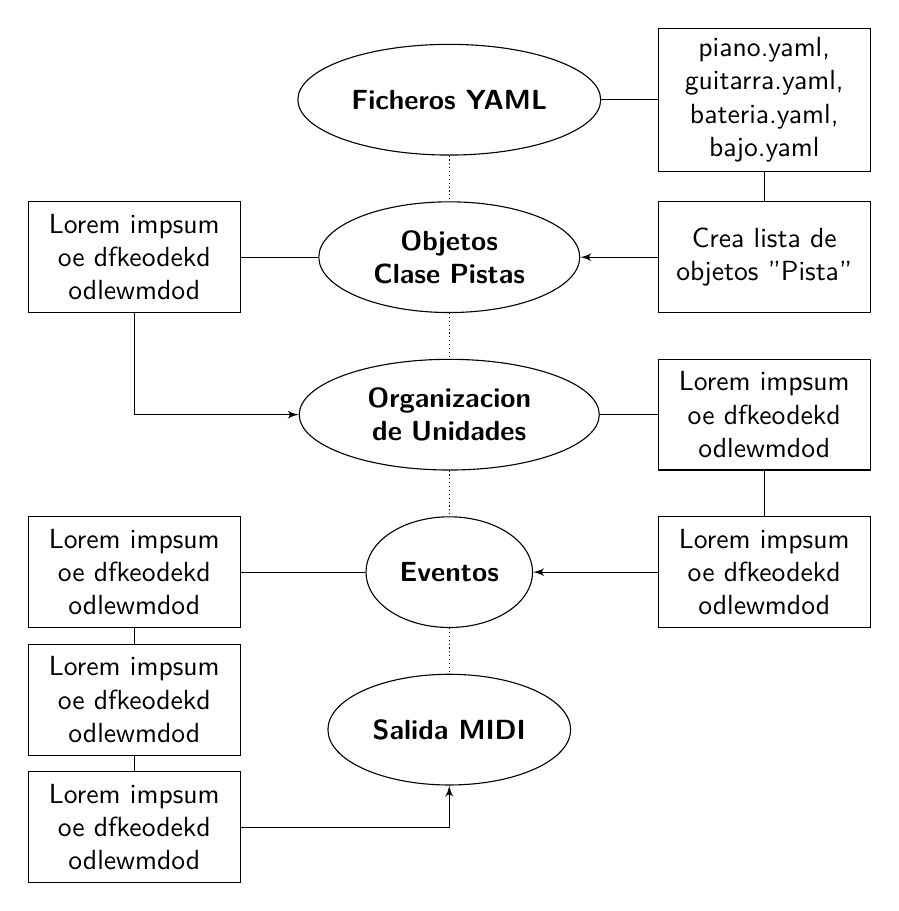
\begin{tikzpicture}[node distance = 2cm, auto]

    \tikzstyle{circulo} = [
        ellipse, 
        draw, 
        %fill=red!20, 
        minimum height=4em,
        text centered, 
        node distance=2cm,
    font=\bfseries
    ]
    \tikzstyle{block} = [
        rectangle, 
        draw, 
        %fill=blue!20, 
        text width=7em, 
        text centered, 
        minimum height=4em,
        node distance=2cm,
    ]
    \tikzstyle{line} = [
        draw,
        -latex',
    ]

    \node [circulo]                               (ana) { Ficheros YAML};
    \node [circulo, text width=6em,below of=ana]  (dis) { Objetos Clase Pistas };
    \node [circulo, text width=7em, below of=dis] (dev) { Organizacion de Unidades };
    \node [circulo, below of=dev]                 (doc) { Eventos };
    \node [circulo, below of=doc]                 (dep) { Salida MIDI };

    \draw[densely dotted] (ana) -- (dis);
    \draw[densely dotted] (dis) -- (dev);
    \draw[densely dotted] (dev) -- (doc);
    \draw[densely dotted] (doc) -- (dep);

    \node [block, 
        right of=ana,
        node distance=4cm,
    ](boc) { 
    piano.yaml,
    guitarra.yaml,
    bateria.yaml,
    bajo.yaml
    };


    \node [block, 
        below of=boc
    ](enc) { 
        Crea lista de objetos "Pista"
    };

    \path [line] (ana) -- (boc) -- (enc) -- (dis);

    \node [block, 
        left of=dis,
        node distance=4cm,
    ](def) { 
        Lorem impsum oe dfkeodekd odlewmdod
    };

    \path [line] (dis) -- (def) |-  (dev) ;

    \node [block, 
        right of=dev,
        node distance=4cm,
    ](per) { 
       Lorem impsum oe dfkeodekd odlewmdod
    };


    \node [block, 
        below of=per
    ](opt) { 
       Lorem impsum oe dfkeodekd odlewmdod
    };

    \path [line] (dev) -- (per) -- (opt) -- (doc);

    \node [block, 
        left of=doc,
        node distance=4cm,
    ](fun) { 
        Lorem impsum oe dfkeodekd odlewmdod
    };

    \node [block, 
        below = 0.2cm of fun
    ](for) { 
        Lorem impsum oe dfkeodekd odlewmdod
    };
    \node [block, 
        below = 0.2cm of for
    ](not) { 
        Lorem impsum oe dfkeodekd odlewmdod
    };

    \path [line] (doc) -- (fun) -- (for) -- (not) -| (dep) ;

    \end{tikzpicture}
     
\end{center}

\newpage

\hypertarget{entrevistas}{%
\subsection{9 Entrevistas}\label{entrevistas}}

Entrevistas del tipo no estructuradas, por pautas y guías.\footnote{Franco
  (2011)}

Pautas / guias :

\begin{itemize}
\item
  Background

  \begin{itemize}
  \item
    Experiencia con representación de información musical textual

    \begin{itemize}
    \tightlist
    \item
      Relación con manipulacion musical a traves de parametros.
    \end{itemize}
  \end{itemize}
\item
  Predisposición a trabajar (leer/escribir) con musica que se encuentre
  descripta en formato textual
\end{itemize}

\newpage

\hypertarget{referencias}{%
\subsection{0 Referencias}\label{referencias}}

reserva de referencias:,\footnote{Allen (1983)},\footnote{Schaeffer
  (1966)}\footnote{Samaruga (2016)},\footnote{Lerdahl y Jackendof (1996)}

\newpage

\hypertarget{bibliografuxeda}{%
\subsection*{10 Bibliografía}\label{bibliografuxeda}}
\addcontentsline{toc}{subsection}{10 Bibliografía}

\hypertarget{refs}{}
\leavevmode\hypertarget{ref-allen}{}%
ALLEN, J.F., 1983. Maintaining knowledge about temporal intervals.
\emph{Communications of the ACM.}, pp. 832-843. ISSN 0001-0782. DOI
\href{https://doi.org/10.1145/182.358434}{10.1145/182.358434}.

\leavevmode\hypertarget{ref-sphinx}{}%
BRANDL, G. y SPHINX TEAM, 2018. Python Documentation Generator. {[}en
línea{]}. Disponible en: \url{https://sphinx-doc.org/en/master}.

\leavevmode\hypertarget{ref-clark}{}%
CLARK, C. y TINDALE, A., 2014. Flocking: A Framework for Declarative
Music-Making on the Web. \emph{The Joint Proceedings of the ICMC and
SMC}, vol. 1, no. 1, pp. 50-57.

\leavevmode\hypertarget{ref-coombs}{}%
COOMBS, J.H., RENEAR, A.H. y DE ROSE, S.J., 1987. Markup Systems and the
Future of Scholarly Text Processing. \emph{Communications of the ACM}
{[}en línea{]}, vol. 30, no. 11, pp. 933-47. DOI
\href{https://doi.org/10.1145/32206.32209}{10.1145/32206.32209}.
Disponible en: \url{http://www.xml.coverpagess.org/coombs.html}.

\leavevmode\hypertarget{ref-music21}{}%
CUTHBERT, M.S., 2018. music21: a toolkit for computer-aided musicology.
{[}en línea{]}. Disponible en: \url{http://web.mit.edu/music21}.

\leavevmode\hypertarget{ref-franco}{}%
FRANCO, Y., 2011. Tesis de Investigación. {[}en línea{]}. Disponible en:
\url{http://tesisdeinvestig.blogspot.com/2011/06/entrevistas.html}.

\leavevmode\hypertarget{ref-good}{}%
GOOD, M., 2001. MusicXML: An Internet-Friendly Format for Sheet Music.
\emph{Proceedings of XML} {[}en línea{]}, Disponible en:
\url{http://michaelgood.info/publications/music/musicxml-an-internet-friendly-format-for-sheet-music/}.

\leavevmode\hypertarget{ref-graham2}{}%
GRAHAM, P., 2001. \emph{Beating the Averages} {[}en línea{]}. 2001.
Estados Unidos: Franz Developer Symposium; www.paulgraham.com.
Disponible en: \url{http://www.paulgraham.com/avg.html}.

\leavevmode\hypertarget{ref-grela}{}%
GRELA, D., 1992. \emph{Análisis Musical: Una Propuesta Metodológica}.
1992. Rosario, Santa Fe, Argentina: Facultad de Humanidades y Artes.
SERIE 5: La música en el Tiempo. Nº1.

\leavevmode\hypertarget{ref-hunt}{}%
HUNT, A. y THOMAS, D., 1999. \emph{The Pragmatic Programmer: From
Journeyman to Master}. S.l.: The Pragmatic Bookshelf. ISBN
\href{https://worldcat.org/isbn/9780201616224}{9780201616224}.

\leavevmode\hypertarget{ref-kernighan}{}%
KERNIGHAN, B.W. y PLAGUER, P.J., 1978. \emph{The Elemenets Of Programing
Style}. Estados Unidos: McGraw-Hill Book Company. ISBN
\href{https://worldcat.org/isbn/9780070342071}{9780070342071}.

\leavevmode\hypertarget{ref-leek}{}%
LEEK, J., 2017. The future of education is plain text. {[}en línea{]}.
Disponible en:
\url{https://simplystatistics.org/2017/06/13/the-future-of-education-is-plain-text}.

\leavevmode\hypertarget{ref-lerdahl}{}%
LERDAHL, F. y JACKENDOF, R., 1996. \emph{A Generative Theory of Tonal
Music}. Estados Unidos: The MIT Press. ISBN
\href{https://worldcat.org/isbn/026262107X}{026262107X}.

\leavevmode\hypertarget{ref-moolenaar}{}%
MOOLENAAR, B., 2000. Seven habits of effective text editing. {[}en
línea{]}. Disponible en: \url{http://moolenaar.net/habits.html}.

\leavevmode\hypertarget{ref-vim}{}%
MOOLENAAR, B., 2018. VIM. {[}en línea{]}. Disponible en:
\url{https://www.vim.org/docs.php}.

\leavevmode\hypertarget{ref-penfold}{}%
PENFOLD, R.A., 1992. \emph{Advanced MIDI Users Guide}. United Kingdom:
PC Publishing. ISBN
\href{https://worldcat.org/isbn/978-1870775397}{978-1870775397}.

\leavevmode\hypertarget{ref-raymond2}{}%
RAYMOND, E.S., 1997. \emph{The Cathedral and the Bazaar}. 1997. Estados
Unidos: Linux Kongress; O'Reilly Media.

\leavevmode\hypertarget{ref-raymond}{}%
RAYMOND, E.S., 1999. \emph{The Art of UNIX Programming}. Estados Unidos:
Addison-Wesley Professional. ISBN
\href{https://worldcat.org/isbn/978-0131429017}{978-0131429017}.

\leavevmode\hypertarget{ref-python}{}%
ROSSUM, G.V., 2018. Python 3.7. {[}en línea{]}. Disponible en:
\url{https://docs.python.org/3/}.

\leavevmode\hypertarget{ref-samaruga}{}%
SAMARUGA, L.M., 2016. \emph{Un modelo de representación y análisis
estructural de la música electroacústica .} Tesis doctoral. S.l.:
Universidad Nacional de Quilmes.

\leavevmode\hypertarget{ref-schaeffer}{}%
SCHAEFFER, P., 1966. \emph{Tratado de los objetos musicales}. S.l.: s.n.
ISBN \href{https://worldcat.org/isbn/9788420685403}{9788420685403}.

\leavevmode\hypertarget{ref-selfridge}{}%
SELFRIDGE-FIELD, E., 1997. \emph{Beyond MIDI: The Handbok of Musical
Codes}. Estados Unidos: The MIT Press. ISBN
\href{https://worldcat.org/isbn/9780262193948}{9780262193948}.

\leavevmode\hypertarget{ref-mml}{}%
STEYN, J., 2001. Music Markup Language. {[}en línea{]}. Disponible en:
\url{https://steyn.pro/mml}.

\leavevmode\hypertarget{ref-git}{}%
TORVALDS, L., 2018. GIT. {[}en línea{]}. Disponible en:
\url{https://git-scm.com/docs}.

\leavevmode\hypertarget{ref-gnu}{}%
VARIOS, A., 2001. ¿Que es el Software Libre? {[}en línea{]}. Disponible
en: \url{https://www.gnu.org/philosophy/free-sw.es.html}.

\leavevmode\hypertarget{ref-pyyaml}{}%
VARIOS, A., 2018a. PyYAML is a full-featured YAML framework for the
Python programming language. {[}en línea{]}. Disponible en:
\url{https://pyyaml.org/}.

\leavevmode\hypertarget{ref-standarlib}{}%
VARIOS, A., 2018b. The Pyhton Standar Library. {[}en línea{]}.
Disponible en: \url{https://docs.python.org/3/library/index.html}.

\leavevmode\hypertarget{ref-yaml}{}%
VARIOS, A., 2018c. YAML Ain't Markup Language. {[}en línea{]}.
Disponible en: \url{http://yaml.org/}.

\leavevmode\hypertarget{ref-wild}{}%
WILD, J., 1996. A Review of the Humdrum Toolkit: UNIX Tools for Musical
Research, created by David Huron. \emph{Music Theory Online}, vol. 2,
no. 7.

\leavevmode\hypertarget{ref-yzaguirre}{}%
YZAGUIRRE, G., 2016. Manifiesto del Laboratorio de Software Libre. {[}en
línea{]}. Disponible en:
\url{https://labsl.multimediales.com.ar/Manifiesto_del_Laboratorio_de_Software_Libre_.html}.

\end{document}
\renewcommand\tabcolsep{4pt}
